\chapter{Grundlagen}
\label{ch:grundlagen}


\section{Konventionelle Projektabwicklung in der deutschen Baupraxis}
\label{sec: 2.1}
Ziel: Der Leser soll die Struktur, die Rollenverteilung und die prozessualen Schwachstellen der traditionellen Projektabwicklung verstehen. Dieses Kapitel etabliert das "Problem", für das die Arbeit eine Lösung präsentiert.

Zielsetzung: Den Leser in das Thema einführen und die prägenden Regelwerke der konventionellen Projektabwicklung in Deutschland benennen.\\
- Feststellung: Die deutsche Baupraxis wird maßgeblich durch HOAI und VOB geformt.\\
- Grundprinzip herausarbeiten: Strikte Trennung von Planungs- und Ausführungsleistungen.\\
- Charakterisierung des Modells: Sequenzieller Ablauf in Phasen.\\



\subsection{Das Prozessmodell - HOAI Leistungsphasen}
\label{sec: 2.1.1}
Zielsetzung: Das abstrakte "Phasenmodell" mit dem konkreten Ablauf der HOAI-Leistungsphasen füllen und dessen starre, lineare Struktur verdeutlichen.\\
- Prozessstruktur: Wird durch die neun Leistungsphasen der HOAI definiert.\\
- Darstellung des Ablaufs: Inhärent linear und sequenziell (LPH 1 -> LPH 9).\\
- Kritischen Punkt identifizieren: Wesentliche Kosten- und Qualitätsentscheidungen fallen in den frühen Planungsphasen (insb. LPH 2-3).\\
- Problem benennen: Zu diesem frühen Zeitpunkt fehlt die vertraglich gebundene Expertise der Ausführung.\\
- Empfehlung: Visualisierung des linearen Ablaufs durch ein einfaches Diagramm.\\

\subsection{Die Organisationsstruktur - getrennte Silos}
\label{sec: 2.1.2}
Zielsetzung: Die prozessuale Trennung auf die organisatorische Ebene übertragen und das Problem der isolierten Akteure (Silos) einführen.\\
- Organisationsstruktur beschreiben: Klassische Dreieckskonstellation (Bauherr, Planer, Ausführender) mit bilateralen Verträgen.\\
- Problem der "Silos" formulieren: Jeder Akteur ist primär auf die Erfüllung des eigenen Vertrags fokussiert.\\
- Kommunikationswege: Oft nur indirekt über den Bauherrn, nicht disziplinübergreifend.\\

\subsection{Die Konsequenzen - strukturelle Schwachstellen}
\label{sec: 2.1.3}
Zielsetzung: Die negativen, systemischen Folgen der beschriebenen Struktur klar benennen und mit Belegen untermauern. Dies ist der Kern der Problemanalyse.\\
- Schwachstellen auflisten und erläutern:\\
- Späte Einbindung von ausführendem Know-how.\\
- Informationsverluste an den Schnittstellen.\\
- Entstehung eines adversialen Projektklimas (Fokus auf Nachtragsmanagement).\\
- Direkte Verbindung zu Kosten- und Terminüberschreitungen herstellen\\

- Zusammenfassen: Das konventionelle Modell bietet zwar einen klaren rechtlichen Rahmen, weist jedoch inhärente Schwächen auf, die Effizienz und Kooperation behindern.
- Schlussfolgerung: Angesichts aktueller Herausforderungen ist das Modell zunehmend reformbedürftig.\\
- Überleitung formulieren: Hinweis auf die Entwicklung alternativer, international etablierter Projektabwicklungsmodelle als Reaktion auf diese Defizite.

\clearpage

\section{Integrierte Projektabwicklungsmodelle als alternativer Ansatz}
\label{sec: 2.2}

% Ziel: Der Leser soll eine Einführung in die Entstehung und Entwicklung integrierter Projekabwicklung bekommen.

\subsection{Lean als Fundament der integrierten Projektabwicklung (\ac{IPA})}
\label{sec:2.2.1}

% Ziel: Vermittlung der Lean-Pilosophie als Ursprungsgedanke und der Weiterentwicklung über Lean Construction zu kollaborativen Projekabwicklungsmodellen
Die im vorangegangenen Abschnitt aufgezeigten Schwachstellen konventioneller, sequenzieller Projektabwicklung sind keineswegs ein neues Phänomen oder eine reine Eigenheit der Bauwirtschaft. Vergleichbare Herausforderungen zeigten sich bereits nach dem Zweiten Weltkrieg in der japanischen Automobilindustrie. Die dort vorherrschenden Produktionsmethoden waren von Ineffizienz und Verschwendung geprägt, was angesichts knapper Ressourcen nicht tragbar war. Als Reaktion darauf entwickelte der Ingenieur Taiichi Ohno bei Toyota einen grundlegend neuen Managementansatz, der heute als das Toyota-Produktionssystem bekannt ist und das Fundament der Lean-Philosophie bildet.

Ursprung des Ansatzes (Lean Management) Skizzieren
- Toyota-Produktionssystem\autocite[]{ohno_toyota-produktionssystem_2013} als Ursprung
- Kernideen und Prinzipien : Wertmaximierung, Verschwendungsreduktion, People First (checken), Kaizen

Transfer auf die Baubranche durch Lean Construction
- Landesweite Aufmerksamkeit in Japan nach der Ölkrise 1973
- Während sich die 
- Internationale Aufmerksamkeit durch 

Ursprung und Entwicklung von Projetct Alliancing, IPD und IPA bis heute

\subsection{Prinzipien und Merkmale der Integrierten Projektabwicklung}
\label{sec:2.2.2}

IPA als ist das organisatorische und vertragliche "Betriebssystem", um die Lean-Philosophie in Bauprojekten praktisch umzusetzen.\\

Schlüsseleigenschaften und IPA-Charakteristika:\\
- Frühzeitige Integration aller Schlüsselpartner (Planer und Ausführende) von Beginn an.\\
Ein Mehrparteienvertrag, der alle Partner an einen Tisch bindet.\\
Ein gemeinsames Risikomanagement (Chancen-/Risikopool).\\
Eine kollaborative Kultur und gemeinsame Entscheidungsfindung.\\


\subsection{Internationale Erfolge und Status Quo in Deutschland}
\label{sec:2.2.3}

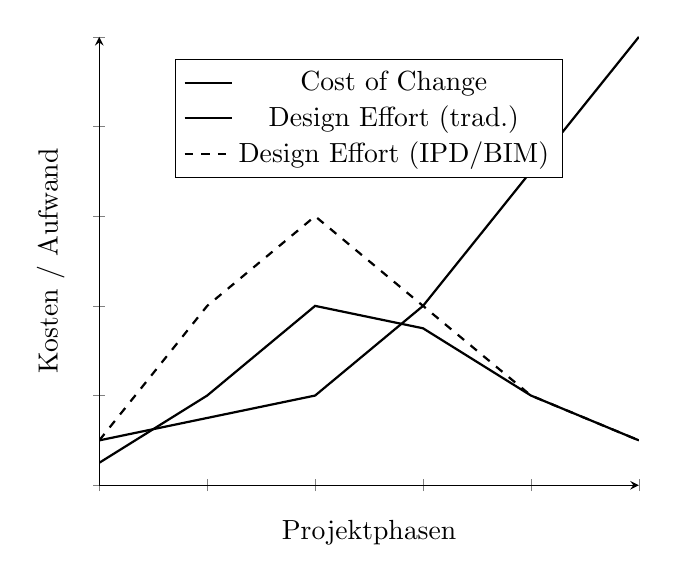
\begin{tikzpicture}
    \begin{axis}[
        xlabel={Projektphasen},
        ylabel={Kosten / Aufwand},
        xmin=0, xmax=10,
        ymin=0, ymax=10,
        xticklabels={},
        yticklabels={},
        axis lines=left,
        legend style={at={(0.5,0.95)},anchor=north},
        ]

        % Cost of change (konventionell)
        \addplot[
            thick,
        ]
        coordinates {(0,1) (2,1.5) (4,2) (6,4) (8,7) (10,10)};
        \addlegendentry{Cost of Change}

        % Level of Effort (konventionell)
        \addplot[
            thick,
        ]
        coordinates {(0,0.5) (2,2) (4,4) (6,3.5) (8,2) (10,1)};
        \addlegendentry{Design Effort (trad.)}

        % Level of Effort (IPD/BIM)
        \addplot[
            thick,
            dashed
        ]
        coordinates {(0,1) (2,4) (4,6) (6,4) (8,2) (10,1)};
        \addlegendentry{Design Effort (IPD/BIM)}

    \end{axis}
\end{tikzpicture}


International: Hohe Erfolgsquoten im angelsächsischen Raum (USA, UK, Australien mit "Project Alliancing") bei der Einhaltung von Kosten und Terminen (Quelle z.B. cook2014).\\

Deutschland: Das Thema gewinnt stark an Fahrt: es gibt eine wachsende Zahl an Pilotprojekten (Quelle: IPA-Report 2024 von haghsheno2025).\\

Eine zentrale Kernmethode zur Kosten- und Wertsteuerung innerhalb dieser IPA-Modelle ist das Target Value Design.\\

\clearpage

\section{Target Value Design (TVD) als Kernmethode}
\label{sec: 2.3}

\subsection{Begriffliche Einordnung und Definition}
\label{sec: 2.3.1}

% =======================================================
% FÜR ABSCHNITT 2.3.1: TVD - Prozess oder Methode
% =======================================================
%   - Ziel: Eine präzise und trennscharfe Definition von TVD für die
%     vorliegende Arbeit herleiten. Es soll geklärt werden, ob TVD als
%     Prozess, als Methode oder als beides zu verstehen ist, um eine
%     eindeutige Basis für die nachfolgende Analyse zu schaffen.
%
%   - Einstieg: Feststellung, dass die Begriffe "Prozess" und "Methode"
%     in der Literatur zu TVD oft unscharf oder synonym verwendet werden.
%
%   - Begriffsdefinition "Methode": Ein systematisches, geplantes Vorgehen,
%     das auf Prinzipien, Regeln und Werkzeugen basiert, um ein Ziel zu erreichen.
%
%   - Begriffsdefinition "Prozess": Eine logische und zeitliche Abfolge von
%     miteinander verknüpften Aktivitäten zur Umwandlung eines Inputs in einen Output.
%
%   - Anwendung auf TVD:
%     - TVD ist mehr als ein reiner Prozess, da es eine bestimmte Denkweise
%       ("Target First"), Prinzipien (Kollaboration) und Werkzeuge voraussetzt.
%     - Diese übergeordnete Denkweise wird jedoch erst durch einen konkreten,
%       strukturierten Ablauf (Prozess) in der Praxis anwendbar.
%
%   - Fazit & Positionierung: Für diese Arbeit wird TVD als eine
%     *MANAGEMENT-METHODE* verstanden, die durch einen
%     _STRUKTURIERTEN PROZESS_ operationalisiert und umgesetzt wird.
%     Diese Definition legitimiert die nachfolgende "prozessorientierte
%     Darstellung" der Methode.
%
% =======================================================

Zur Hinleitung auf die in \cref{ch:methodik} beschriebene, methodische Vorgehensweise soll an dieser Stelle auf das in dieser Arbeit zu Grunde liegende Verständnis von \ac{TVD} als Prozess bzw. Methode eingegangen werden.\\
In der Literatur ist die Abgrenzung zwischen Prozess und Methode in der aktuellen Diskussion um TVD unscharf. Folgt man dem Ergebnis einer einfachen Stichwortsuche in einschlägigen wissenschaftlichen Datenbanken (z.B. reseachgate.net) so wird schnell deutlich, das in der überwiegenden Mehrheit der Literatur (ca. 70\%) Target Value Design als Prozess verstanden wird.
Glenn Ballard, der als einer Gründer des \ac{TVD} gilt, bezeichnet letzteres hingegen häufig als Managementansatz bzw. Management-Methode \autocite[]{}.\\
% In der allgemeinen Literatur wird ein Prozess als

- Definition Prozess Vs. Methode: Verständnis als Management Methode die durch einen sturkturierten Prozess umgesetzt wird -> legitimiert die nachfolgende prozessoroentierte Darstelung.\\

\subsection{Historische Entwicklung}
\label{sec: 2.3.2}

Inhalt: Herleitung aus den drei historischen Strängen (vgl. Ballard, 2025, Kap. 3 ):\\
Manufacturing: Target Costing bei Toyota (Produktionssystem) .\\
UK: Cost Planning der Quantity Surveyors (1950er) .\\
Finnland: Haahtela-Modell (1980er) .\\
USA: Die Synthese zu "Lean TVD" (ab 2000er) .\\
Ziel: Kosten als Inputgröße statt Outputgröße der Planung.\\

\subsection{Handlungslogik und Kernprinzipien}
\label{sec: 2.3.3}

Target First: Kosten sind eine Design-Voraussetzung, kein Ergebnis.\\

Collaboration: Alle sitzen früh in einem Boot (Cross-funktionale Teams).\\

Optimize the Whole: Projektziel vor Einzelziel.\\

Continuous Improvement: Der Prozess ist nie "fertig", sondern wird iterativ verbessert.\\



\subsection{Methoden und Werkzeuge}
\label{sec: 2.3.4}

Die operative Umsetzung der Zielkostenerreichung erfordert spezifische Methoden, die über die reine Kooperationsbereitschaft (vgl. \cref{sec: 2.2}) hinausgehen. Nach Ballard (2012) stützt sich der TVD-Prozess auf ein integriertes Set an Werkzeugen, welche die Designstrategie, die Entscheidungsfindung und die technische Datenverarbeitung steuern.\autocite[vgl. S. 15]{ballard_target_2012}

\subsection*{Set-Based-Design}
Set-Based Design (SBD): Definition als paralleles Entwickeln von Alternativen bis zum "Last Responsible Moment" (vgl. Ballard, 2025, S. 27; LCI 2016).

\subsection*{Choosing By Advantages}
Choosing By Advantages (CBA): Definition als Entscheidungsmethode basierend auf Vorteilen, nicht Gewichtungen

\subsection*{A3-Methode bzw. Report}
A3 Thinking / Reports: Definition als Problemlösungs- und Konsens-Werkzeug.

\subsection*{Last Planner System}
Last Planner System (LPS) in der Planung: Nutzung zur Steuerung des Design-Workflows (nicht nur Bau).

\subsection*{Building Information Modelling}
Im TVD-Kontext wird \ac{BIM} zur Datenbank für die Kostenkalkulation.\\
Zweck: "Wir müssen alle 3 Wochen wissen, was es kostet."
Funktion: Automatisierter Massenauszug (Quantity Take-Off). Wenn Sie eine Wand im Modell verschieben, ändert sich sofort die m²-Zahl in der Datenbank.\\
Ziel: Geschwindigkeit..\\


\subsection{Akteure und Organisationsstruktur}
\label{sec: 2.3.5}

- Unterschied zu Target Costing (Industrie) und Value Engineering (klassische Planung).\\

- Einordnung in IPA-Kontext.\\

- Relevanz: Warum TVD nicht nur Kostentechnik, sondern Führungsprinzip ist.\\

- TVD als prozessorientierte Managementmethode mit systematischer Kosten- und Wertsteuerung.\\

Zur detaillierten Untersuchung dieses Prozesses im Kontext der deutschen Baupraxis wird im folgenden Kapitel das methodische Vorgehen beschrieben. Dabei wird zunächst das Forschungsdesign erläutert und anschließend dargelegt, wie der idealtypische TVD-Prozess systematisch analysiert und modelliert wird.

\clearpage